\documentclass[aspectratio=169]{beamer}

% Suppress all navigation symbols
\setbeamertemplate{navigation symbols}{}
\setbeamertemplate{headline}{}
\setbeamertemplate{footline}{}
\setbeamertemplate{itemize items}[circle]
\setbeamertemplate{footline}[frame number]

\setbeamercolor{structure}{fg=blue}
\setbeamercolor{normal text}{fg=black, bg=white}
\setbeamerfont{title}{series=\bfseries, size=\Huge}
\setbeamerfont{frametitle}{series=\bfseries, size=\LARGE}

\setbeamertemplate{footline}{
  \begin{tikzpicture}[remember picture,
                      overlay,
                      shift={(current page.south west)}]
    \node [black!50, inner sep=2mm, anchor=south east]
          at (current page.south east)
          {\large \bfseries \insertframenumber};
  \end{tikzpicture}
}

\definecolor{red}{RGB}{220, 50, 47}
\definecolor{green}{RGB}{133, 153, 0}
\definecolor{cyan}{RGB}{42, 161, 152}
\definecolor{blue}{RGB}{38, 139, 210}
\definecolor{yellow}{RGB}{181, 137, 0}

\usepackage{fontspec}
\setsansfont{Overpass}[Scale=MatchLowercase]
\setmonofont{Overpass Mono}[Scale=MatchLowercase]

\usepackage{listings}
\lstset{
  basicstyle=\ttfamily\small,
  commentstyle={\color{black!50}},
  language=Java,
}

\usepackage{pgfplots}

\usepackage{tikz}
\usetikzlibrary{arrows}
\usetikzlibrary{backgrounds}
\usetikzlibrary{calc}
\usetikzlibrary{decorations.pathreplacing}
\usetikzlibrary{fit}
\usetikzlibrary{positioning}
\usetikzlibrary{matrix}
\usetikzlibrary{scopes}
\usetikzlibrary{shapes}
\usetikzlibrary{tikzmark}
\usetikzmarklibrary{listings}

\tikzset{
    arrow/.style={->,>=stealth', shorten >=2pt, thick},
    box/.style = {
      minimum size=0.6cm,
      rounded corners,
      rectangle,
      fill=blue!50
    },
    bigbox/.style = {
      draw=blue!50,
      thick,
      fill=blue!10,
      rounded corners,
      rectangle
    },
}


\title{JDebloat: Tutorial}
\author{Jon Eyolfson}
\date{2020-07-10}

\setbeamertemplate{title page}
{
  \begin{tikzpicture}[remember picture,
                      overlay,
                      shift={(current page.south west)}]
    \node (title) [inner sep=0, scale=1.2, align=center]
          at (\paperwidth / 2, \paperheight * 2 / 3)
          {\usebeamerfont{title}\usebeamercolor[fg]{title} \inserttitle};
    \node (author) [node distance=0.2em, scale=1, below=of title]
          {\insertauthor};

    \node (onrtitle) [scale=1.25] at (\paperwidth / 2, \paperheight / 3)
          {Synergistic Software Customization: Framework, Algorithms, and Tools};

    \node (onrauthor) [scale=1, node distance=0.2em, below=of onrtitle]
          {N00014-18-1-2037 (PI: Miryung Kim, co-PIs: Jens Palsberg and Harry Xu)};
    \node [node distance=0, below=of onrauthor]
          {\includegraphics[scale=0.1]{ucla-logo.eps}};
    

    \node [anchor=south east, inner sep=2mm] at (\paperwidth, 0)
          {\bfseries \insertdate};
  \end{tikzpicture}
}

\begin{document}

  \begin{frame}[plain]
    \titlepage
  \end{frame}

  \setcounter{framenumber}{0}

  \begin{frame}
    \centering
    \includegraphics[scale=0.3]{pi-overview.png}
  \end{frame}

  \begin{frame}
    \frametitle{We Provide a Pre-built Docker Image}

    The URL for the latest image is:

    \url{http://debloating.cs.ucla.edu/dist/jdebloat_image.tgz}

    (followed by \texttt{docker load -i jdebloat\_image.tgz})

    \vspace{1em}

    There is also a Dockerfile, if you would like to build it yourself:

    \url{http://debloating.cs.ucla.edu/dist/Dockerfile}

    \vspace{3em}

    For this tutorial we'll use the latest image and start it using:

    \texttt{docker run -it jdebloat}

  \end{frame}

  \begin{frame}
    \frametitle{Push-Button Debloating}

    \begin{center}
      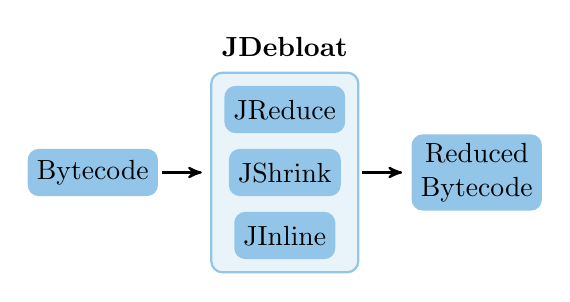
\begin{tikzpicture}[
        outer sep=0.05cm,
        node distance=0.8cm
      ]
        \tikzstyle{bigbox} = [
          draw=blue!50,
          thick,
          fill=blue!10,
          rounded corners,
          rectangle
        ]
        \tikzstyle{box} = [
          minimum size=0.6cm,
          rounded corners,
          rectangle,
          fill=blue!50
        ]

        \node[box] (1) {JReduce};
        \node[box,below of=1] (2) {JShrink};
        \node[box,below of=2] (3) {JInline};

        \begin{pgfonlayer}{background}
          \node[bigbox] [fit = (1) (3)] (jdebloatbox) {};
        \end{pgfonlayer}

        \node[box, left=of 2.west, anchor=east] (input) {Bytecode};
        \node[box, right=of 2.east, anchor=west, align=center] (output) {Reduced\\Bytecode};

        \draw[arrow] (input.east) -- (jdebloatbox);
        \draw[arrow] (jdebloatbox.east) -- (output.west);

        \node [above of=1] {\bfseries JDebloat};
      \end{tikzpicture}
    \end{center}

    \vspace{2em}

    Just run \texttt{./jdebloat -h} for a list of commands.

    \vspace{1em}

    By default all tools run together, however you may run them individually.
  \end{frame}

  \begin{frame}
    \frametitle{Directory Layout}

    \hspace{1em}
    \begin{itemize}
      \item[] {\bfseries \texttt{data}} --- Where to add benchmarks, and customize them.
      \vspace{1em}
      \item[] {\bfseries \texttt{output}} --- All \texttt{run} commands output files here.
      \vspace{1em}
      \item[] {\bfseries \texttt{results}} --- Summary results of the 25 default benchmarks.
      \vspace{1em}
      \item[] {\bfseries \texttt{scripts}} --- Internal code used to call the tools.
      \vspace{1em}
      \item[] {\bfseries \texttt{tools}} --- Source code of all individual tools.
    \end{itemize}
  \end{frame}

  \begin{frame}
    \frametitle{Adding a New Benchmark is One Line}

     Add the repository and commit to run in \texttt{data/benchmarks.csv}.

     \vspace{3em}

     For this tutorial we'll add Maven Wrapper (\texttt{https://github.com/takari/maven-wrapper}).
  \end{frame}

  \begin{frame}
    \frametitle{New Benchmarks Require Maven and Tests}

    Our framework automatically builds projects using \texttt{mvn} and extracts test cases.

    \vspace{1em}

    We use \textit{Surefire Report Plugin} to get a list of test classes.

    \vspace{3em}

    We list all test classes in \texttt{output/benchmark-id/initial/test.classes.txt}.

    \vspace{1em}

    Our tools assume all test cases should pass, to exclude any class add the class name to
    \texttt{data/excluded-tests.txt} (separated by newlines).
  \end{frame}

  \begin{frame}
    \frametitle{Our Tools Require Setup}

    In our image, our tools are pre-built and setup.

    \vspace{3em}

    However, if you would like to start from scratch:

    \vspace{1em}

    \hspace{2em} Remove all tools, and benchmark data using \texttt{./jdebloat.py clean}.

    \vspace{1em}

    \hspace{2em} Setup all the tools, ready to run the benchmarks using \texttt{./jdebloat.py setup}.
  \end{frame}

  \begin{frame}
    \frametitle{Running JDebloat}

    After setup, running \texttt{./jdebloat.py run} executes the tools in different combinations.

    \vspace{3em}

    Each benchmark has a corresponding directory in \texttt{output/benchmark-id}, with the following subdirectories:

    \vspace{1em}

    \begin{itemize}
      \item[] {\bfseries \texttt{benchmark}} --- Source code for the benchmark.
      \vspace{1em}
      \item[] {\bfseries \texttt{initial}} --- Initial JAR files without modifications.
      \vspace{1em}
      \item[] {\bfseries \texttt{initial+tool(s)}} --- JAR files after running tool(s), in order.
    \end{itemize}

    \vspace{1em}

    Each subdirectory with JAR files contains a \texttt{stats.csv} file with size statistics.
  \end{frame}

  \begin{frame}
    \frametitle{JReduce: A Dynamic Java Bytecode Reducer}

    Focus on buggy input reduction to decompilers, instead of tree-shaking.

    \vspace{1em}

    Extended idea to remove methods and fields (instead of classes).

    \vspace{3em}

    Run with \texttt{./jdebloat run jreduce}.
  \end{frame}

  \begin{frame}
    \frametitle{JReduce Uses Tests to Remove Code}
    \centering
    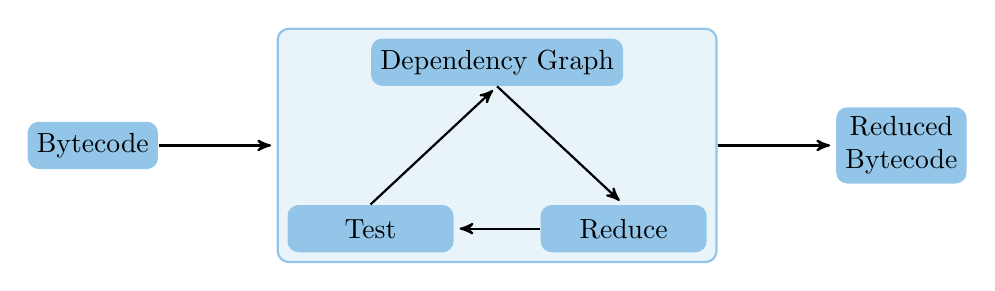
\begin{tikzpicture}
      \node [box] (dependencygraph) {Dependency Graph};

      \node [
        box,
        minimum width=6em,
        below=1.5cm and .75cm of dependencygraph.south west,
      ] (test) {Test};

      \node [
        box,
        minimum width=6em,
        below=1.5cm and .75cm of dependencygraph.south east,
      ] (reduce) {Reduce};

      \draw[arrow] (dependencygraph.south) -- (reduce.north);
      \draw[arrow] (reduce.west) -- (test.east);
      \draw[arrow] (test.north) -- (dependencygraph.south);

      \begin{pgfonlayer}{background}
        \node[draw, bigbox,fit=(dependencygraph) (test) (reduce)] (outline) {};
      \end{pgfonlayer}

      \node [box, left=1.5cm of outline] (input) {Bytecode};
      \node [box, right=1.5cm of outline, align=center] (output) {Reduced\\Bytecode};

      \draw[arrow] (input.east) -- (outline.west);
      \draw[arrow] (outline.east) -- (output.west);
    \end{tikzpicture}
  \end{frame}

  \begin{frame}
    \frametitle{JShrink Removes Unused Code Through Analysis}

    JShrink performs 4 transformations:
    \begin{enumerate}
      \item Unused method removal
      \item Unused field removal
      \item Static inlining
      \item Class collapsing / class hierarchy specialization
    \end{enumerate}

    \vspace{2em}

    Builds a static call graph, and handles reflection by adding dynamic
    information

    \vspace{3em}

    Run with \texttt{./jdebloat.py run jshrink}.
  \end{frame}

  \begin{frame}
    \frametitle{JShrink Uses Call Graph Analysis to Reduce Code Size}

    \centering
    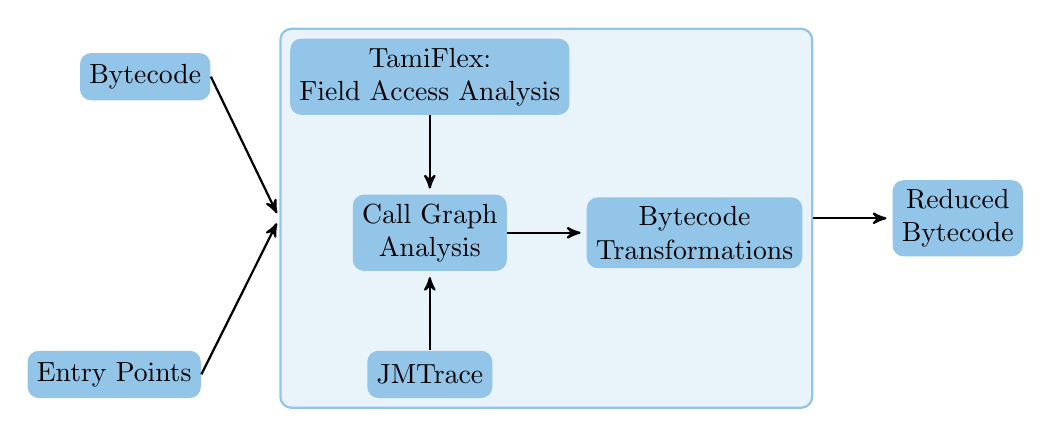
\begin{tikzpicture}
      \node[box, align=center] (cga) {Call Graph\\Analysis};
      \node[box, right=of cga, align=center] (bytecodetransformations) {Bytecode\\Transformations};
      \node[box, above=of cga, align=center] (tamiflex) {TamiFlex:\\Field Access Analysis};
      \node[box, below=of cga] (jmtrace) {JMTrace};

      \draw[arrow] (tamiflex) -- (cga.north);
      \draw[arrow] (cga) -- (bytecodetransformations);
      \draw[arrow] (jmtrace) -- (cga.south);

      \begin{pgfonlayer}{background}
        \node[draw, bigbox, fit=(cga) (bytecodetransformations) (tamiflex) (jmtrace)] (jshrink) {};
      \end{pgfonlayer}

      \node[box, left=of tamiflex] (inputbc) {Bytecode};
      \node[box, left=2.1cm of jmtrace, align=center] (entrypoints) {Entry Points};

      \node[box, right=of jshrink, align=center] (output) {Reduced\\Bytecode};

      \draw[arrow] (jshrink.east) -- (output.west);
      \draw[arrow] (inputbc.east) -- (jshrink.west);
      \draw[arrow] (entrypoints.east) -- (jshrink.west);
    \end{tikzpicture}

    \vspace{1em}
    Accepted to \textbf{ESEC/FSE 2020}, individual artifact available at \url{https://doi.org/10.6084/m9.figshare.12435542}.
  \end{frame}

  \begin{frame}[fragile]
    \frametitle{JInline Finds Call Sites to Inline}

    We replace a method call with the method body

    \vspace{1em}

    Allows us to remove the method (and maybe even library)

    \vspace{3em}

    Run with \texttt{./jdebloat.py run jinline}.

  \end{frame}

  \begin{frame}[fragile]
    \frametitle{JInline Uses Program Behavior to Inline Code}

    \centering
    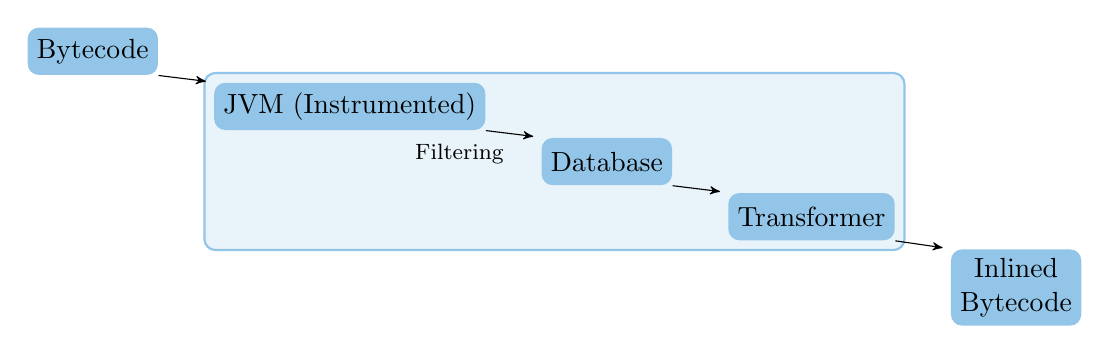
\begin{tikzpicture}[
      node distance=0.7cm, ->, >=stealth', shorten >=1mm
    ]
      \node [box] (original) {Bytecode};
      \node [box, right=of original, yshift=-0.7cm] (jvm) {JVM (Instrumented)};
      \node [box, right=of jvm, yshift=-0.7cm] (database) {Database};
      \node [box, right=of database, yshift=-0.7cm] (jinliner)
            {Transformer};
      \node [box, right=of jinliner, yshift=-0.9cm, align=center] (modified) {Inlined\\Bytecode};

      \begin{pgfonlayer}{background}
        \node[draw, bigbox, fit=(jvm) (database) (jinliner)] (jinline) {};
      \end{pgfonlayer}

      \path (original.south east) edge (jvm.north west)
            (jvm.south east) edge
              node [below left] {\footnotesize Filtering} (database.north west)
            (database.south east) edge (jinliner.north west)
            (jinliner.south east) edge (modified.north west);
    \end{tikzpicture}

  \end{frame}

  \begin{frame}
    \frametitle{Running All Tools}

    Simply run: \texttt{./jdebloat.py run} for all combinations.

    \hspace{1em} or run: \texttt{./jdebloat.py run jinline jshrink jreduce} for our best combination.

    \vspace{3em}

    Compare the output of \texttt{output/benchmark-id/initial+tool(s)} to

    \hspace{1em} \texttt{output/benchmark-id/initial}, specifically \texttt{stats.csv}.

  \end{frame}

\end{document}
